%!TeX program = xelatex
\documentclass[11pt]{article}

\usepackage{graphicx}
\usepackage{fancyhdr}
\usepackage{geometry}
\usepackage[utf8]{inputenc}
\usepackage{enumitem}
\usepackage{amsmath} 
\usepackage{multirow}
\usepackage{caption}
\usepackage{float}
\usepackage{fontspec}
\usepackage{cite}
\usepackage{listings}
%\setmainfont{UT Sans}
\usepackage{geometry}
\usepackage{xcolor}

\lstdefinestyle{customc}{
	belowcaptionskip=1\baselineskip,
	breaklines=true,
	frame=L,
	xleftmargin=\parindent,
	language=C,
	showstringspaces=false,
	basicstyle=\large\ttfamily,
	keywordstyle=\bfseries\color{green!40!black},
	commentstyle=\itshape\color{purple!40!black},
	identifierstyle=\color{blue},
	stringstyle=\color{orange},
}

\lstset{escapechar=@,style=customc}

\geometry{a4paper,left=20mm,right=20mm,total={160mm,220mm}}
\pagestyle{fancy}
\thispagestyle{plain}
\fancyheadoffset{0cm}
\rhead{\textit{Andrei Vasilcoi}\\Grupa 4452}

\renewcommand*\contentsname{Cuprins}
\renewcommand*\tablename{Tab.}
\renewcommand*\figurename{Fig.}
\renewcommand\refname{Bibliografie}
\renewcommand{\theenumi}{\Alph{enumi}}
\author{Andrei Vasilcoi}
\newcommand{\EqRow}{\vspace{1.5mm}}
\begin{document}
\begin{titlepage}

\newcommand{\HRule}{\rule{\linewidth}{0.5mm}}
	
\begin{center}
	%autor si indrumator mai jos
\textsc{\LARGE Universitatea Transilvania din Brașov}\\[0.5cm]

\includegraphics[width=0.25\textwidth]{logo_ut.jpg}\\[0.5cm]
\textsc{\Large Facultatea de Inginerie Electrică și Știința Calculatoarelor}\\[0.5cm]
\textsc{\large Departament Automatică și Informatică Aplicată}\\[1.5cm]
\HRule\\[0.5cm]
{\Large Proiect \textit{Sisteme inteligente de control}}\\[0.5cm]
{\LARGE\bfseries Tema nr. 59}\\[0.5cm]
\HRule\\[2.5cm]
\begin{minipage}{1\textwidth}
	\begin{flushleft}
		\large
		\textit{Autor}\\
		Andrei \textsc{Vasilcoi}\\
	\end{flushleft}
\end{minipage}
~
\end{center}
\centering
\vspace{5cm}
{\large Mai 2019, Brașov}\\[5cm]
\end{titlepage}

\newpage
\pagenumbering{arabic}
\tableofcontents

\newpage	
\section{Tema proiectului}
Se va proiecta un regulator fuzzy pentru controlul unui proces descris de funcția de transfer:
\EqRow
\begin{equation} 
G_p(s)=\frac{K_p}{(sT_{1}+1)(sT_{2}+1)}
\EqRow
\end{equation}
Se va realiza o implementare a regulatorului proiectat, în limbajul C/C++, care ulterior se va testa pentru diverse valori ale mărimilor de intrare ale sistemului de inferență prin comparație cu funcționarea aceluiași sistem de inferențe realizat în Matlab.

\begin{center}
\captionof{table}{Date de proiectare}
\begin{tabular}{|c|c|c|c|c|c|c|c|}
	\hline
	{\multirow{2}{*}{Tema nr.} } &  \multicolumn{3}{ c| }{Parametrii procesului} & {\multirow{2}{*}{$M_{v}$}} & {\multirow{2}{*}{$t_{s}$}} & {\multirow{2}{*}{$e_{st}$}} &{\multirow{2}{*}{Student}} \\ \cline{2-4}
	&$K_p$ & $T_{1}$ & $T_{2}$ & & &  &\\ 
	\hline
 \multirow{2}*{59} & \multirow{2}*{1} & \multirow{2}*{120} & \multirow{2}*{5} &\multirow{2}*{4\%} &\multirow{2}*{120} & \multirow{2}*{0\%} & \multirow{2}*{Vasilcoi S. Andrei} \\ &&&&&&& \\
	\hline
\end{tabular}
\end{center}

\section{Indicații și recomandări}
\begin{enumerate}[label=\alph*)]
	\item Proiectarea și analiza sistemului de reglare se va face folosind mediul Matlab-Simulink. Implementarea în program se va face doar după determinarea sistemului de inferențe cu care se obțin performanțele impuse.
	\item Nu sunt impuse restricții pentru tipul regulatorului fuzzy sau tipul inferențelor utilizate, decât aceea că alegerea acestora trebuie să conducă la obținerea performanțelor.
	\item Programul realizat va fi testat prin comparație cu funcționarea sistemului implementat în mediul Matlab. Se vor lua diverse valori ale variabilelor de intrare ale sistemului de inferență pentru care se vor înregistra valorile de ieșire obținute în Matlab și cele obținute cu ajutorul programului.
\end{enumerate}
\section{Conținutul minimal al proiectului}
\begin{enumerate}[label=\alph*)]
	\item Enunțul și descrierea problemei.
	\item Prezentarea sistemului de reglare și a structurii regulatorului fuzzy ales. Obs: Se va justifica alegerea tipului de regulator.
	\item Prezentarea sistemului de inferență obținut (variabile fuzzy, funcții de apartenență, reguli, tipul inferenței fuzzy, caracteristica statică, metoda de defuzzificare – dacă este cazul – etc.). Obs: Se vor justifica toate alegerile referitoare la sistemul de inferență.
	\item Prezentarea rezultatelor simulării sistemului de reglare proiectat (Matlab-Simulink).
	\item Prezentarea particularităților de implementare, utilizate la realizarea programului.
	\item Se vor anexa schema Simulink și programul realizat.
\end{enumerate}
\section{Condiții pentru susținerea proiectului}
\begin{enumerate}[label=\alph*)]
	\item Proiectul va fi prezentat și susținut. Se vor adresa întrebări referitoare la noțiuni de bază și aspecte întâlnite în realizarea lui.
	\item Proiectul predat trebuie să conțină: redactarea (format electronic și printat), fișierele obținute cu ajutorul aplicației de editare a sistemelor de inferență fuzzy, schemele Simulink, codul sursă al programului și fișierul executabil.
	\item Proiectul poate fi predat până la data examenului scris.
\end{enumerate}
\newpage
\section{Considerații teoretice}
\subsection{Introducere in logica Fuzzy}
Abordarea inginerească „clasică”, strictă, a realităţii este una în special cantitativă, bazată pe
modelări matematice exprimate în forme care inspiră exactitatea. Într-o astfel de abordare,
aprecierea de ordin calitativ a mărimilor, valorilor, rezultatelor etc. este greu interpretabilă,
deoarece acestea au valori stricte, bine precizate. Într-un context strict, modelele disponibile
sunt exacte (de fapt cât mai exacte posibil, cu aproximări şi supoziţii), iar sistemele de
comandă şi control sunt dezvoltate în strânsă legătură cu acestea.
\\
Aplicaţiile practice în domeniul ingineriei electrice, bazate pe teoria mulţimilor fuzzy, între
care şi controlul fuzzy, includ un mecanism de evaluare numerică a aprecierilor calitative,
proprii exprimării uzuale ale experienţei. Abordarea problemelor se extinde, incluzând şi
aprecieri calitative ale rezultatelor.
\\
Aplicaţiile curente în inginerie şi mai exact în control automat apelează doar o parte restrânsă a teoriei mulţimilor fuzzy, care se dovedeşte relativ uşor accesibilă.
\\
O propoziţie fuzzy simplă este o sintagmă de forma “ este ”, în care x este o variabilă fuzzy, iar A este un termen lingvistic (atribut) ce poate caracteriza variabila. Prin analogie, o propoziţie strictă este descrisă printr-o egalitate . Propoziţiile fuzzy conţin cuvântul “este”, care ţine loc semnului “=” din relaţiile stricte.
\\
Valoarea de adevăr a propoziţiei fuzzy este descrisă de funcţia de apartenenţă a mulţimii fuzzy A, adică, pentru o valoare strictă putem preciza în ce măsură “ este ” prin valoarea lui .
\subsection{Interferente de tip Sugeno-Takagi}
În unele aplicaţii practice concrete, procedura stabilirii unei baze de reguli poate consta într-o procesare a unui set de date non-fuzzy (reale). Finalitatea acestei prelucrări ar putea fi transpunerea acestor date într-o formă lingvistică. Datele non-fuzzy sunt obţinute prin înregistrarea semnalelor utile pentru proiectare - mărime de comandă, mărime de reacţie şi/sau eroare de reglare – şi prin calcularea derivatelor acestora, în funcţie de structura de reglare aleasă. Însă extragerea regulilor fuzzy în forma “dacă ... atunci ...” este considerată dificilă din cauză faptului că nu există proceduri sistematizate.
\\
Obţinearea regulilor este strâns legată de mecanismul de inferenţă utilizat.
Dacă un set de date reale privind funcţionarea procesului este disponibil, se poate adapta mecanismul de inferenţă fuzzy de tip Tagaki, într-o formă utilă şi adecvată datelor numerice. Această adaptare reuşeşte să reducă din volumul de calcule al metodelor de inferenţă obişnuite, prin introducerea unei reprezentări mai degrabă numerice a regulilor fuzzy, care în final nu mai sunt deloc evidenţiate.
\\
Forma generală a regulilor fuzzy de tip Sugeno este:
\begin{equation} 
daca \ x_1 \ este \ A_{11} \  si \ x_2 \ este \ A_{21} \ este \ atunci \ y_1 = f_1(x_1, x_2),
\EqRow
\end{equation}

unde $y_1$ este o valoare crisp (singleton, reală). De obicei $f_1(x_1, x_2)$ este un polinom cu variabilele $x_1$ şi $x_2$ de forma $y_1 = p_1x_1 +q_1x_2+ r_1$.
$p_1$, $q_1$ si $r_1$ sunt constante (date, cu valori cunoscute).\\
Indicele inferior 1 se referă la numărul regulii într-o bază de reguli.\\
O regulă fuzzy Sugeno poate fi:
\begin{itemize}
	\item de ordinul zero (daca $p_i,q_i=0$)
	\item de ordinul unu (daca $p_i$ sau $q_i \ne 0$)
	\item de ordinul doi (daca $p_i$ sau $q_i \ne 0$)
\end{itemize}

\subsection{Structura sistemului de reglare}
Se consideră structura clasică de reglare, cu un singur regulator principal, aflat pe calea directă a sistemului. Această structură permite o comparaţie uşoară a performanţelor regulatoarelor fuzzy cu cele ale regulatoarelor clasice, evident pe baza cunoştinţelor prealabile necesare de ingineria reglării automate.\\
Structura de reglare convenţională este un sistem cu reacţie negativă, considerată unitară pentru o simplificare iniţială. Pe calea de reacţie este preluată mărimea de ieşire a părţii fixe $y(t)$, care practic este un semnal achiziţionat corespunzător mărimii supuse reglării. Mărimea de ieşire măsurată este comparată cu o mărime de referinţă $r(t)$, care defineşte evoluţia dorită în timp a sistemului, iar diferenţa celor două reprezintă eroarea de reglare:\\
\begin{equation} 
e(t) = r(t) – y(t)
\EqRow
\end{equation}
\begin{figure}[H]
	\centering
	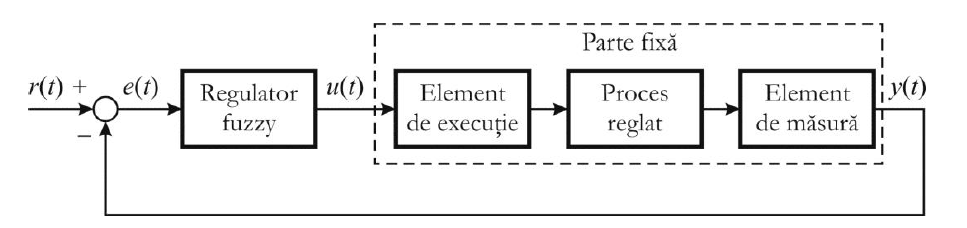
\includegraphics[width=0.7\linewidth]{struct_reg.png}
	\captionof{figure}{Structura conventionala de reglare}
	\label{fig:test2}
\end{figure}

\subsection{Structura regulatorului fuzzy}
Regulatoarele fuzzy sunt una din aplicaţiile importante a teoriei mulţimilor fuzzy. Un sistem de reglare cu regulator fuzzy are principalul avantaj al faptului că permite toleranţă la incertitudine şi imprecizie, aspect demonstrat de numeroase aplicaţii practice.
În varianta clasică, un regulator fuzzy are structura minimală descrisă în figura urmatoare.
\begin{figure}[H]
	\centering
	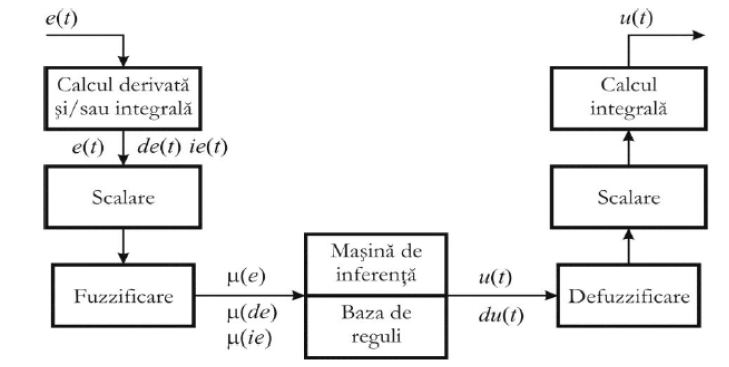
\includegraphics[width=0.5\linewidth]{struct_reg_teorie.png}
	\captionof{figure}{Schema regulatorului fuzzy}
	\label{fig:test2}
\end{figure}
\newpage
\section{Rezolvare}

Am ales regulator fuzzy de tip PD ce foloseste inferente de tip Sugeno-Takagi.
Legea de reglare a regulatoarelor convenţionale este:
\begin{equation} 
u=K_p*e+K_d*d_e
\EqRow
\end{equation}
Unde $K_d=T_d$// Remarcăm aici faptul că la regulatoarele fuzzy, ca de altfel şi la cele numerice, nu este necesară filtrarea care se introduce la regulatoarele analogice din motive de realizabilitate fizică a acestora. Considerente similare vom avea şi în cazul regulatoarelor fuzzy (numerice) PID.

\begin{figure}[H]
	\centering
	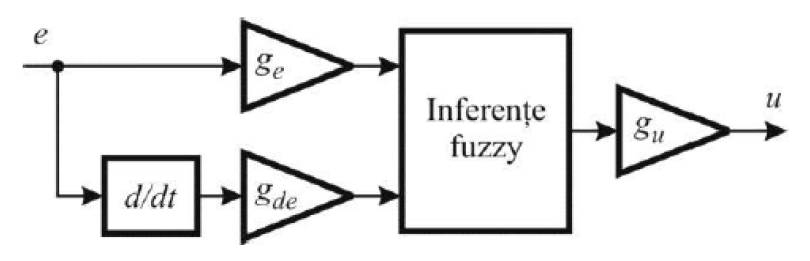
\includegraphics[width=0.4\linewidth]{schema_pid.PNG}
	\captionof{figure}{Schema regulator fuzzy PID}
	\label{fig:test2}
\end{figure}

Variabilele lingvistice pentru un regulator fuzzy PD vor fi:
\begin{itemize}
	\item eroarea
	\item derivata erorii
	\item comanda
\end{itemize}
O regulă tipică din bază are acum formularea:\\
Dacă e este E și de este DE atunci u este U.\\
Regulatorul a fost ales pe baza experimentelor,regulatorul PD fiind cel care a oferit rezultatele cele mai bune.\\
Regulatorul fuzzy primește ca intrare eroarea și derivată erorii iar la ieșire va indica mărimea de comandă,universul de discurs este [-1,1].\\
Eroarea(e) este compusă din 5 funcții de apartenență de tipul triunghi :
\begin{figure}[H]
	\centering
	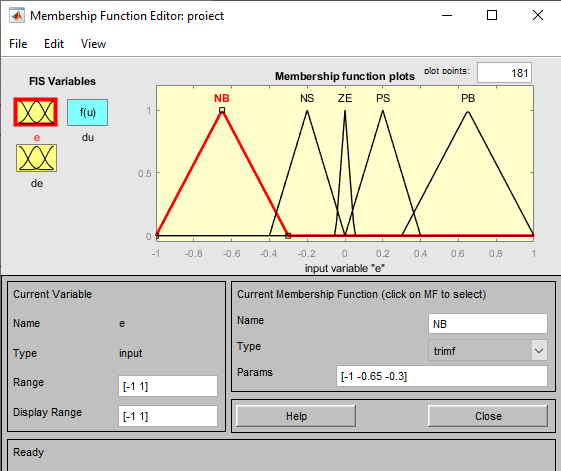
\includegraphics[width=0.5\linewidth]{var_e.PNG}
	\captionof{figure}{Functiile de apartenenta ale erorii}
	\label{fig:test2}
\end{figure}
Derivata erorii(de) este definită de 3 funcții de de apartenență de tip triunghi.
\begin{figure}[H]
	\centering
	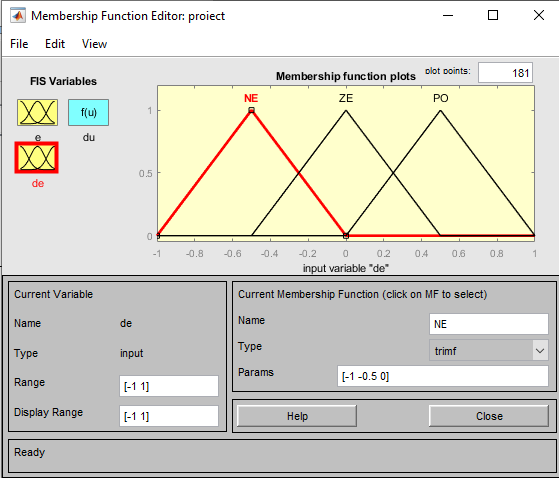
\includegraphics[width=0.5\linewidth]{var_de.PNG}
	\captionof{figure}{Functiile de apartenenta ale derivatei erorii}
	\label{fig:test2}
\end{figure}
Iesirera sistemului, mărimea de comandă, este definită prin 5 valori constate coresunzatoare combinatiilor celor 2 marimi de intrare:
\begin{figure}[H]
	\centering
	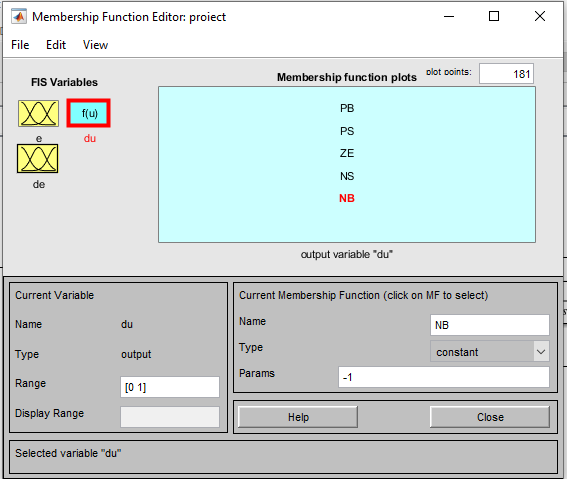
\includegraphics[width=0.5\linewidth]{iesire.PNG}
	\captionof{figure}{Valorile marimii de iesire}
	\label{fig:test2}
\end{figure}
Avand:
\begin{itemize}
	\item PB = 1
	\item PS = 0.5
	\item ZE = 0
	\item NS = -0.5
	\item NB = -1
\end{itemize}
Baza de reguli este aleasă experimental pe baza considerațiilor dobândite în cadrul cursului:
\begin{figure}[H]
	\centering
	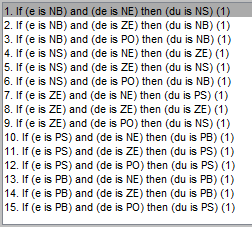
\includegraphics[width=0.4\linewidth]{rules.PNG}
	\captionof{figure}{Baza de reguli a regulatorului fuzzy}
	\label{fig:test2}
\end{figure}
Schema bloc de reglare folosita:
\begin{figure}[H]
	\centering
	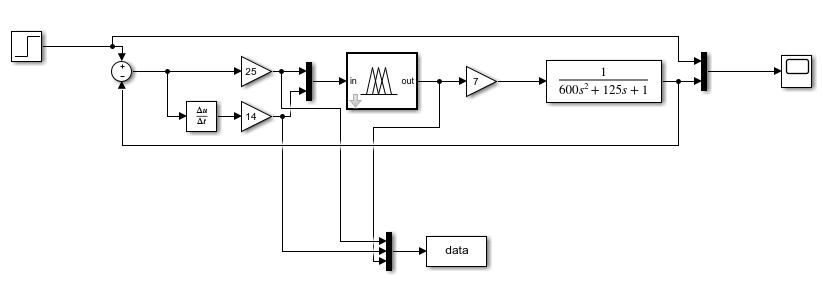
\includegraphics[width=1\linewidth]{schema_sim.PNG}
	\captionof{figure}{Schema sistemului de reglare in Simulink}
	\label{fig:test2}
\end{figure}
Parametrii de simulare au fost determinați pe baza rezultatelor experimentale, astfel că sistemul se încadrează în specificațiile de proiectare impuse inițial.
Parametrii impusi sunt:
\begin{itemize}
	\item Eroarea staționară maximă $e_{st} = 0\%$
	\item Suprareglajul maxim $M_v = 4\%$
	\item Timpul de stabilire maxim $t_s = 120s$
\end{itemize}
Performantele obtinute de sistemul de reglare:
\begin{itemize}
	\item Eroarea staționară maximă $e_{st} = 0\%$
	\item Suprareglajul maxim $M_v = 3\%$
	\item Timpul de stabilire maxim $t_s = 56s$
\end{itemize}
\begin{figure}[H]
	\centering
	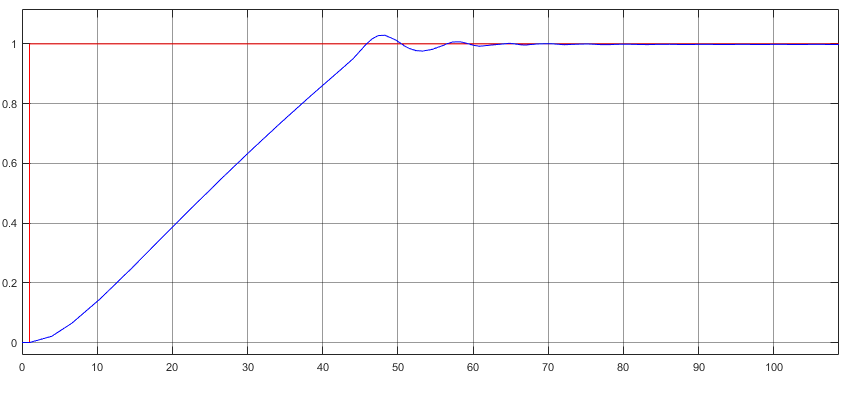
\includegraphics[width=1\linewidth]{diagrama.PNG}
	\captionof{figure}{Graficul semnalului de iesire}
	\label{fig:test2}
\end{figure}
Implementarea regulatorului fuzzy a fost realizată în Microsoft Visual Studio 2017, în limbajul de programare C++, în Tabelul 1.1 se regăsește o paralelă între câteva valori aleatoare determinate în Matlab și cele determinate în programul de implementare.
\newpage

\nocite{*}
\bibliographystyle{ieeetr}
\bibliography{bibliografie}

\end{document}